\section{Mediciones}

\subsection{Banco de medición}

En la figura \ref{fig:banco_medicion} puede observarse un diagrama del banco de
medición. Consiste de los siguientes bloques:

\begin{itemize}
    \item Placa FPGA: genera un pulso cuadrado unipolar, de frecuencia y ciclo
      de trabajo configurables. Con la frecuencia se controla la $PRF$ de los
      pulsos de salida, y con el ciclo de trabajo los valores de tensión del
      pulso de salida del \textit{driver}.
    \item Fuente de alimentación: provee la alimentación $V_{dd}$ para el
      driver. El valor de esta tensión determina la amplitud pico a pico del
      pulso de salida del \textit{driver}.
    \item \textit{Driver}: cumplía la función de \textit{buffer} para la
      \textit{FPGA}, presentando una alta impedancia a la salida de la misma.
      Convierte el pulso unipolar de \qty{3.3}{\volt} en uno bipolar, con
      amplitud pico a pico igual a $V_{dd}$ (\qty{5}{\volt} o \qty{7}{\volt}).
    \item \textit{Pulser}: el \textit{DUT}, genera pulsos ultra cortos en base 
      a la salida del driver.
    \item Osciloscopio: instrumento de medición del experimento. Actúa como
      carga con su impedancia de entrada de \qty{50}{\ohm}.
\end{itemize}

\begin{figure}
  \centering
    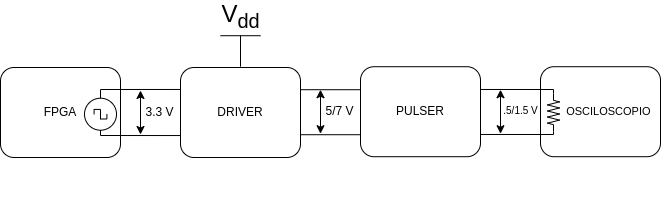
\includegraphics[width=1\textwidth]{images/banco_medicion.drawio.png}
    \caption{Banco de medición}
    \label{fig:banco_medicion}
\end{figure}

\subsubsection{Fuente de alimentación}

Para la fuente de alimentación se utilizó una \textit{Marconi Instruments
TF2154}, en la figura \ref{fig:mediciones_fuente} puede observarse la misma.

Presentaba limitación de corriente regulable e indicadores para la amplitud y la
corriente suministrada, lo que permitía trabajar de manera segura, dentro de los
límites de consumo obtenidos en las simulaciones anteriores
\textcolor{red}{REEMPLAZAR ESTA REF \ref{TODO}}.

Como fuese explicado en la sección \textcolor{red}{REEMPLAZAR ESTA REF
\ref{TODO}},
la corriente máxima esperada en las condiciones de trabajo era menor a \qty{200}{\milli\ampere},
por lo que se monitoreó durante todo el experimento que la corriente entregada por la fuente
no supere este máximo teórico.

\begin{figure}
  \centering
    \includegraphics[width=0.3\textwidth]{images/mediciones_fuente.png}
    \caption{Fuente de alimentación \textit{Marconi Instruments TF2154}.}
    \label{fig:mediciones_fuente}
\end{figure}


\subsubsection{FPGA}

La \textit{FPGA} generaba el pulso unipolar cuadrado de entrada, que controla la
$PRF$ y el ciclo de trabajo del pulso del driver. La placa utilizada fue
\textit{Nexys-4 DDR} de Digilent \cite{digilent_nexys4ddr}, con un chip
\textit{Artix-7} de Xilinx. En la figura \ref{fig:mediciones_fpga} puede
observarse la misma. 

Se utilizó una \textit{FPGA} para poder validar la utilidad del prototipo en el
contexto de un sistema UWB como el descripto en \ref{}, en el que se dispone de
señales de control digitales. Este componente del sistema es fácilmente
reemplazable por otra \textit{FPGA} o sistema embebido.

Las variables de ajuste del pulso unipolar de la \textit{FPGA} eran las siguientes

\begin{itemize}
  \item Frecuencia: la frecuencia de la señal cuadrada de entrada es igual a la
    frecuencia de repetición de pulsos ($PRF$) del sistema, ya que controla la
    frecuencia con la que el \textit{SRD} se prende y se apaga y, por lo tanto,
    la frecuencia de generación de pulsos.
  \item Ciclo de trabajo: el ciclo de trabajo de la señal cuadrada unipolar
    determina los extremos de tensión de la señal cuadrada bipolar de salida del
    driver. A mayor ciclo de trabajo, valores más negativos. Este control se da
    a través del control del valor medio de la señal, que luego es restado por
    el capacitor serie del \textit{driver}.
\end{itemize}

\begin{figure}
  \centering
    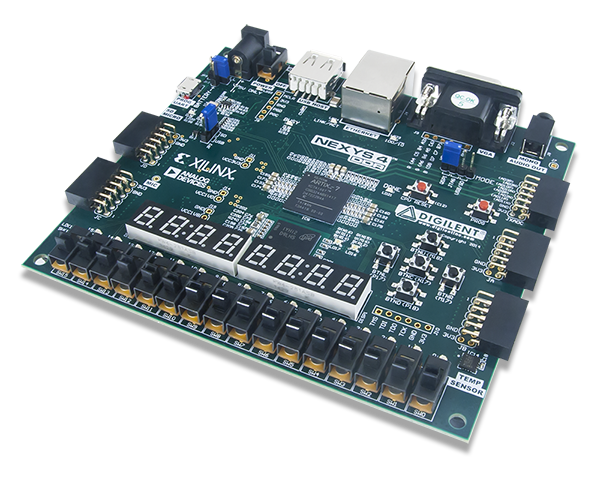
\includegraphics[width=0.4\textwidth]{images/mediciones_fpga.png}
    \caption{Placa de desarrollo \textit{Nexys-4 DDR}.}
    \label{fig:mediciones_fpga}
\end{figure}

\paragraph{Diseño implementado}

El diseño implementado en la \textit{FPGA} consistía en un generador de cuadrada con
ciclo de trabajo y frecuencia variables. La interfaz del sistema consistió en

\begin{itemize}
  \item Los botones \textit{BTNL} y \textit{BTNR} controlaban el ciclo de
    trabajo en pasos de a \qty{1}{\percent} en incrementos y decrementos
    respectivamente.
  \item Los botones \textit{BTND} y \textit{BTNU} controlaban el ciclo de
    trabajo en pasos de a \qty{10}{\percent} en incrementos y decrementos
    respectivamente.
  \item Con los \textit{switches} \textit{SW0} a \textit{SW1} se controlaba la
    frecuencia del pulso unipolar.
    \begin{itemize}
      \item Con \textit{SW0} seleccionado, la frecuencia era de
        \qty{1}{\mega\hertz}.
      \item Con \textit{SW1} seleccionado, la frecuencia era de
        \qty{5}{\mega\hertz}.
      \item Con \textit{SW2} seleccionado, la frecuencia era de
        \qty{10}{\mega\hertz}.
    \end{itemize}
\end{itemize}

En el anexo \ref{app:verilog} se encuentra el \textit{HDL} del diseño implementado.

\subsubsection{Osciloscopio}

El osciloscopio fue utilizado para realizar la medición en el dominio del tiempo
del pulso generado. Para una medición exitosa, era indispensable que este
instrumento cuente con los requerimientos de ancho de banda del pulso. Como fuese
explicado en \textcolor{red}{REEMPLAZAR ESTA REF \ref{TODO}}, el ancho de banda
esperado para el pulso era de \qty{3.6}{\giga\hertz}.

El osciloscopio utilizado fue \textit{Tektronix MSO 70404C}, en la figura 
\ref{fig:osciloscopio} puede observarse el mismo. El instrumento posee 
\qty{4}{\giga\hertz} de ancho de banda analógico, y una tasa de muestreo
de \qty[per-mode=symbol]{25}{\giga\siemens\per\second}, con la posibilidad de
realizar muestreo en tiempo equivalente \cite{oscilloscope_datasheet}. Estas
prestaciones eran suficientes para medir el pulso de salida.

El instrumento posee configuraciones de impedancia de entrada seleccionables entre
\qty{50}{\ohm} y \qty{500}{\mega\ohm} \cite{oscilloscope_datasheet}. Para la
medición del prototipo, se seleccionó la entrada de \qty{50}{\ohm}, actuando
esta impedancia como carga del generador de pulsos.

\begin{figure}
  \centering
    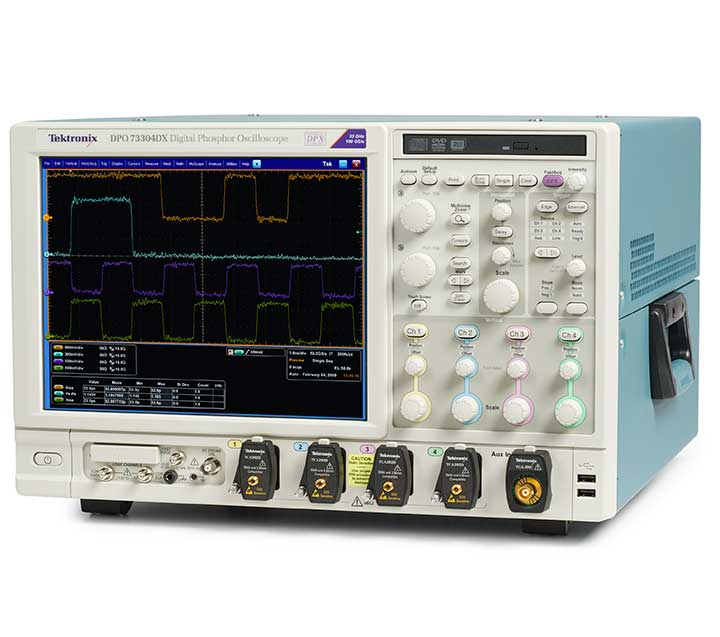
\includegraphics[width=0.4\textwidth]{images/osciloscopio.png}
    \caption{Osciloscopio \textit{Tektronix MSO 70404C}}
    \label{fig:osciloscopio}
\end{figure}

\paragraph{Seguridad del instrumento}

Debido a las prestaciones del osciloscopio, era fundamental garantizar la
integridad del mismo en la medición del protipo. Dado que actuaba como carga del
\textit{DUT}, se debía garantizar que bajo todas las condiciones de
trabajo, la potencia entregada por el generador de pulsos se encuentre dentro de
los límites determinados por el fabricante del equipo para evitar posibles daños.

La máxima tensión de entrada se especifica en $5 \ V_{RMS}$ para una resolución
$\geq \ 100 \ mV/div$ y $1 \ V_{RMS}$ para una resolución $< \ 100 \ mV/div$.
Para garantizar la seguridad del equipo en cualquier caso, se toma como límite
el valor de peor caso, $1 \ V_{RMS}$ (correspondiente a una resolución $\geq \
100 \ mV/div$, para resoluciones menores a esta el límite es mayor).

En condiciones normales de funcionamiento, la potencia disipada por la carga es
mínima, ya que es la potencia que disipa el tren de pulsos en un carga de
\qty{50}{\ohm}. Como fuese desarrollado en \textcolor{red}{REEMPLAZAR ESTA REF
\ref{TODO}}, esta potencia está acotada por
\textcolor{red}{\qty{9999}{\milli\watt}}, que en \qty{50}{\ohm} resultan en
\textcolor{red}{$9999 \ V_{rms}$}, que se encuentran muy por debajo de los $1 \
V_{RMS}$ especificados por el fabricante.

No solo es necesario analizar la disipación de potencia en condiciones normales
de funcionamiento, sino también para el caso de una falla, ya que el principal
objetivo es garantizar la integridad del instrumento en cualquier condición.

En caso de ocurrir alguna falla con algún componente del circuito, el \textit{stub}
de salida provee una función de protección. Este componente, para señales con
una variación temporal mucho mayor al largo del mismo, actúa como una puesta a
tierra.

Entonces, la componente de continua a la salida del generador de pulsos tiene un
valor esperado de \qty{0}{\volt}, tanto para condiciones normales de 
funcionamiento como en presencia de fallas.

En cuanto a la componente alterna de la salida, su valor esperado es
extremadamente bajo, ya que únicamente señales de gran ancho de banda pueden ser
filtradas y permanecer con una amplitud considerable a la salida del 
\textit{stub}.

\subsection{Mediciones realizadas}

Las mediciones consistieron en mediciones en el dominio del tiempo del pulso de
salida. Utilizando funciones provistas por el osciloscopio, se midieron tiempo
de crecimiento, tiempo de decaimiento, amplitud máxima, y ancho a medio máximo
(\textit{FWHM} del inglés \textit{Full Width at Half Maximum}).

Se realizaron distintas mediciones para distintas condiciones de trabajo del
circuito. Se barrió para el pulso digital de entrada, el ciclo de trabajo, y
para la fuente de alimentación distintos valores de tensión.

\begin{itemize}
    \item Para la amplitud de la fuente, se utilizaron valores de \qty{5}{\volt} y
        \qty{7}{\volt}.
        \begin{itemize}
            \item \qty{5}{\volt} por ser un valor fácilmente obtenible en los
                sistemas \textit{UWB} de referencia.
            \item \qty{7}{\volt} por ser la máxima amplitud tolerable por el circuito.
                Tensiones de alimentación mayores a estas resultan en corrientes de
                polarización mayores a las máximas admisibles dado los
                dimensionamientos de las pistas de los \textit{PCBs}.
        \end{itemize}
    \item El ciclo de trabajo se barrió entre \qty{50}{\percent} y
        \qty{70}{\percent}.
        \begin{itemize}
            \item Se tomo 50\% como límite inferior por ser un valor fácilmente
                obtenible como división de un reloj digital.
            \item Se tomo 70\% como límite superior ya que se observó que valores
                superiores a este resultaban en un pulso bipolar con amplitudes
                negativas decrecientes, y por lo tanto, amplitudes de pulso
                decrecientes.
            \item La teoría no indicaba un límite superior para el ciclo de
                trabajo. Sin embargo, este se observó en la práctica debido a no
                idealidades en el pulso de salida del driver, que no era
                perfectamente cuadrado.
        \end{itemize}
\end{itemize}

En la figura \ref{fig:sistema_medido} puede observarse el \textit{pulser} junto con el
\textit{driver} y la \textit{FPGA}.

\begin{figure}
  \centering
    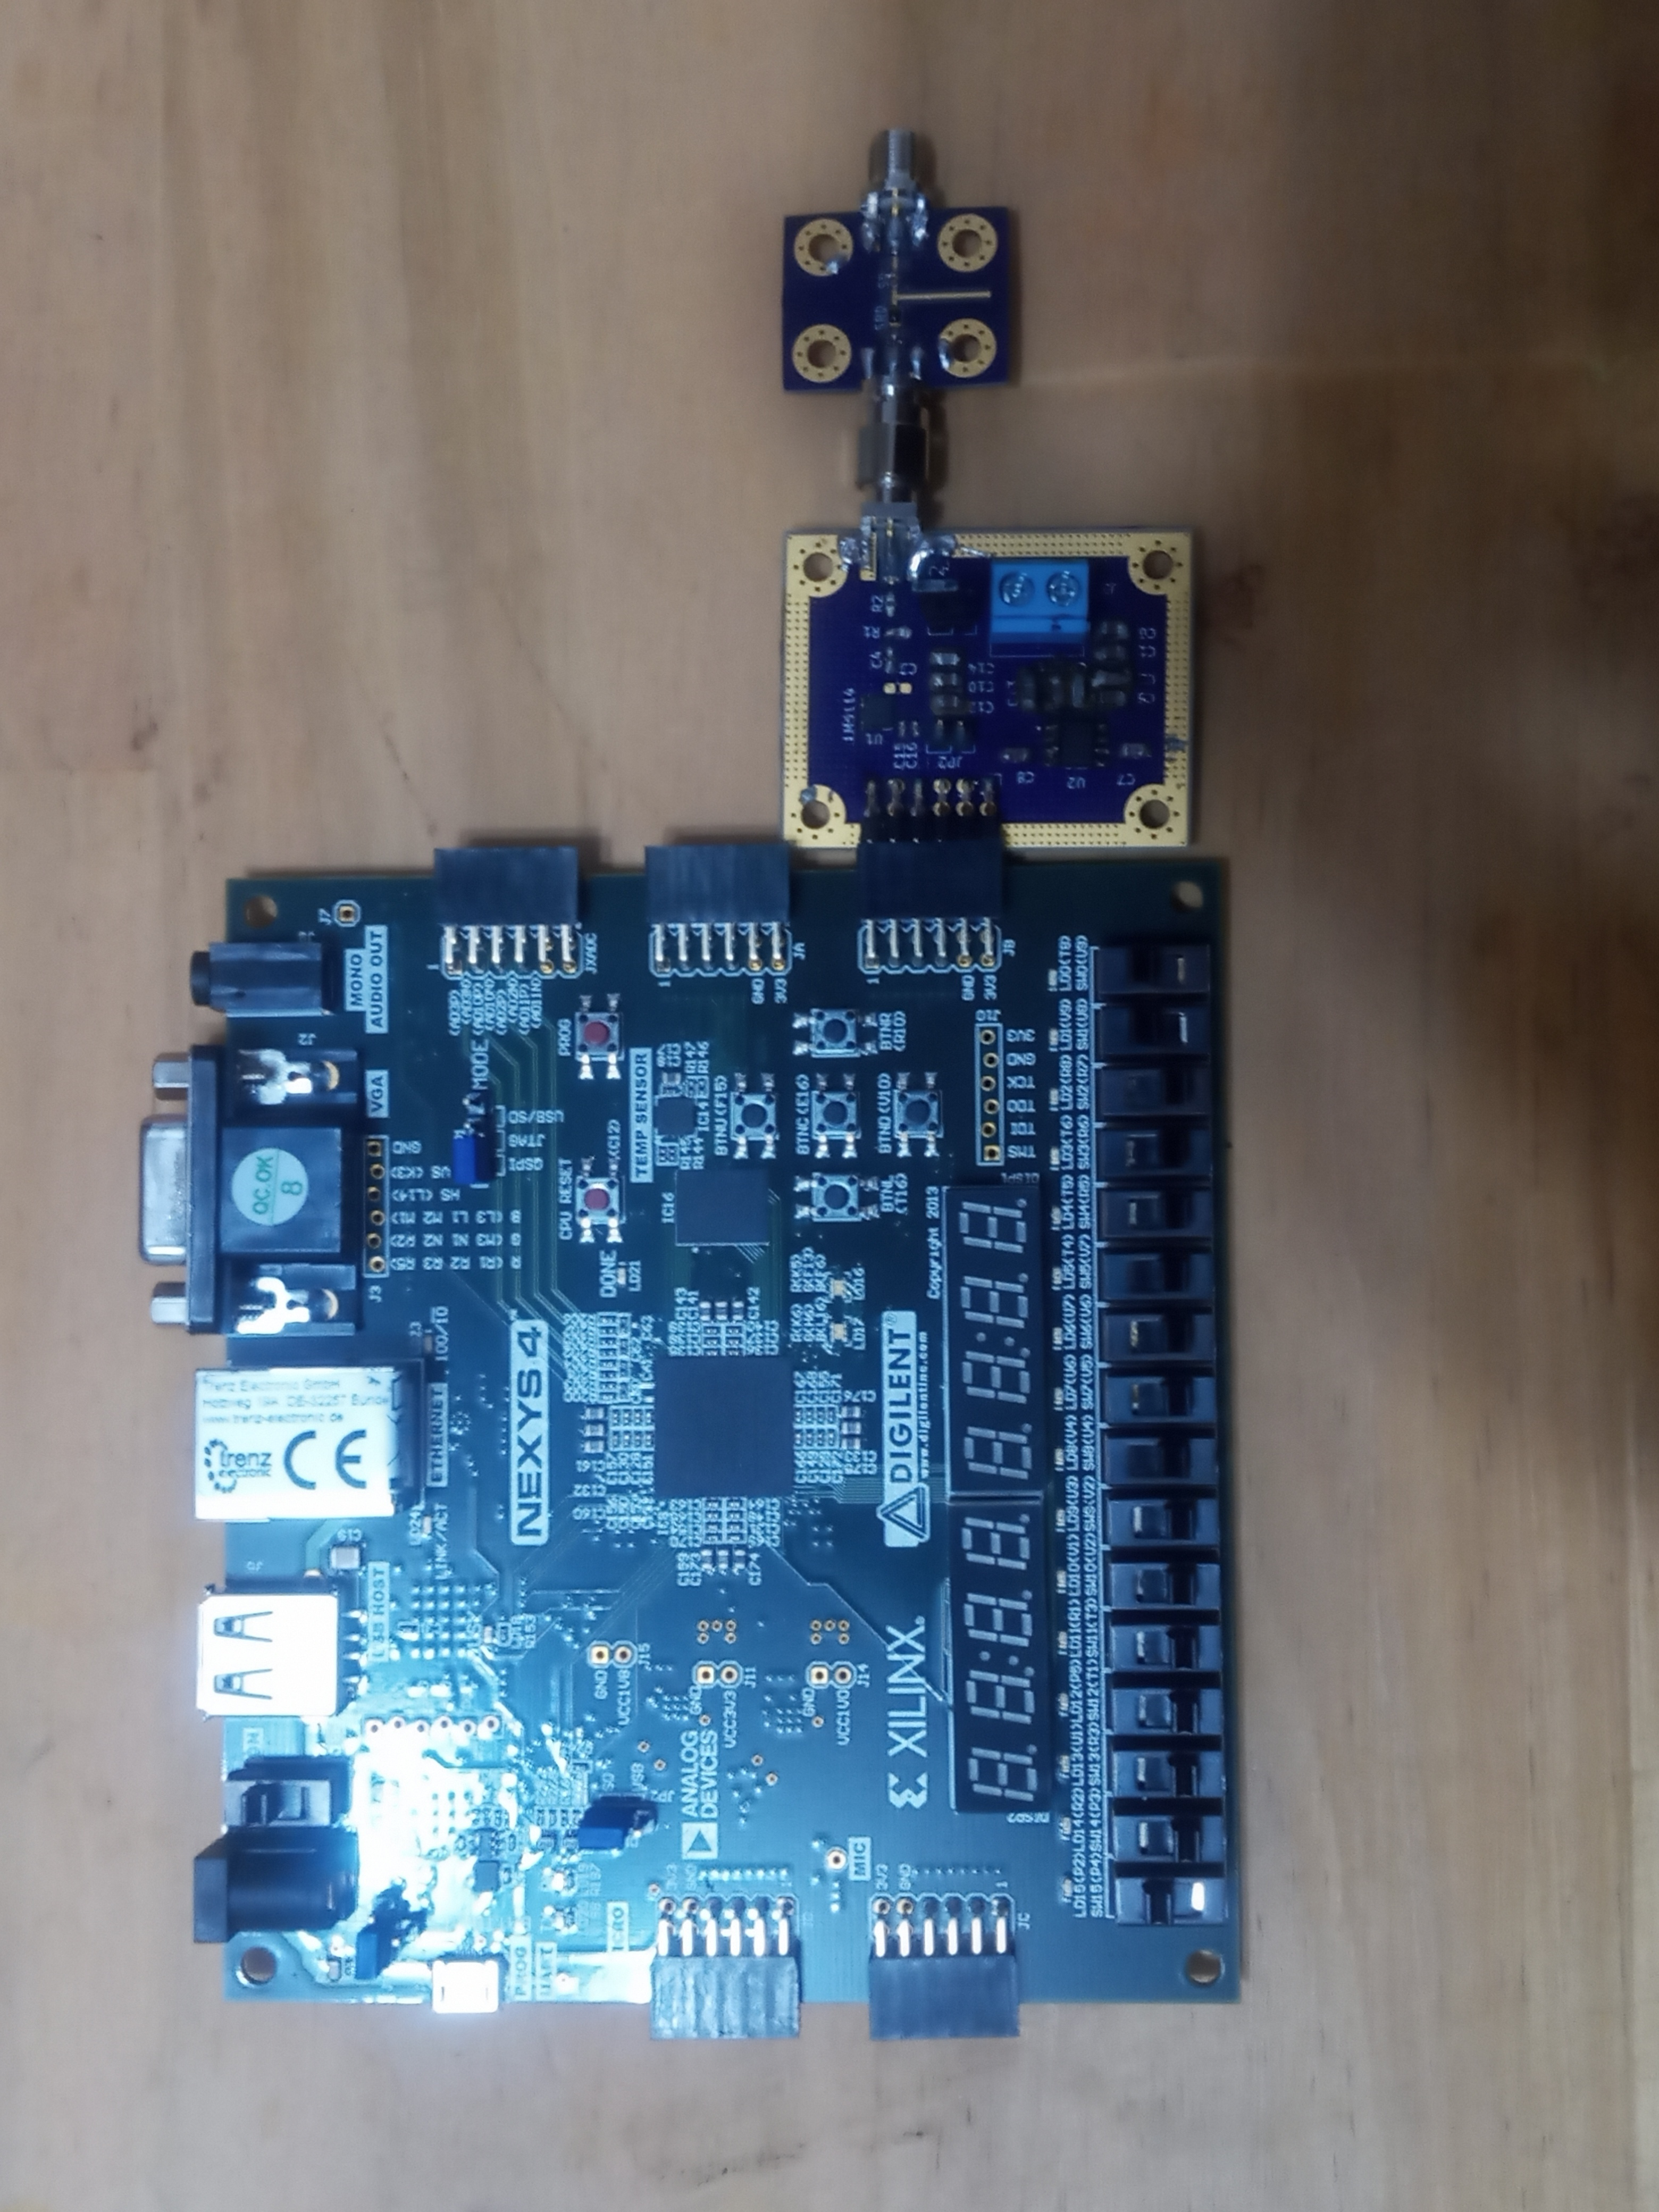
\includegraphics[width=0.4\textwidth]{images/sistema_medido.jpg}
    \caption{\textit{FPGA}, \textit{driver} y \textit{pulser}.}
    \label{fig:sistema_medido}
\end{figure}

\subsubsection{Mediciones preliminares}

Previo a las mediciones principales, se realizó una medición de la salida del driver,
con el objetivo de validar el pulso bipolar generado.

El motivo de esta medición previa, fue la limitada disponibilidad del
osciloscopio de gran ancho de banda utilizado para la medición final del pulso.
Esta pre-medición del pulso bipolar se realizó con un osciloscopio de bajo ancho
de banda, ya que el objetivo era validar los niveles de tensión del pulso, y su
correcta variación con la variación del ciclo de trabajo del pulso unipolar.

En la figura \ref{fig:banco_pre_mediciones} puede observarse el banco de
medición. Los resultados fueron los esperados y, por lo tanto, no se requirió
ninguna iteración sobre la implementación del driver.

\begin{figure}
  \centering
    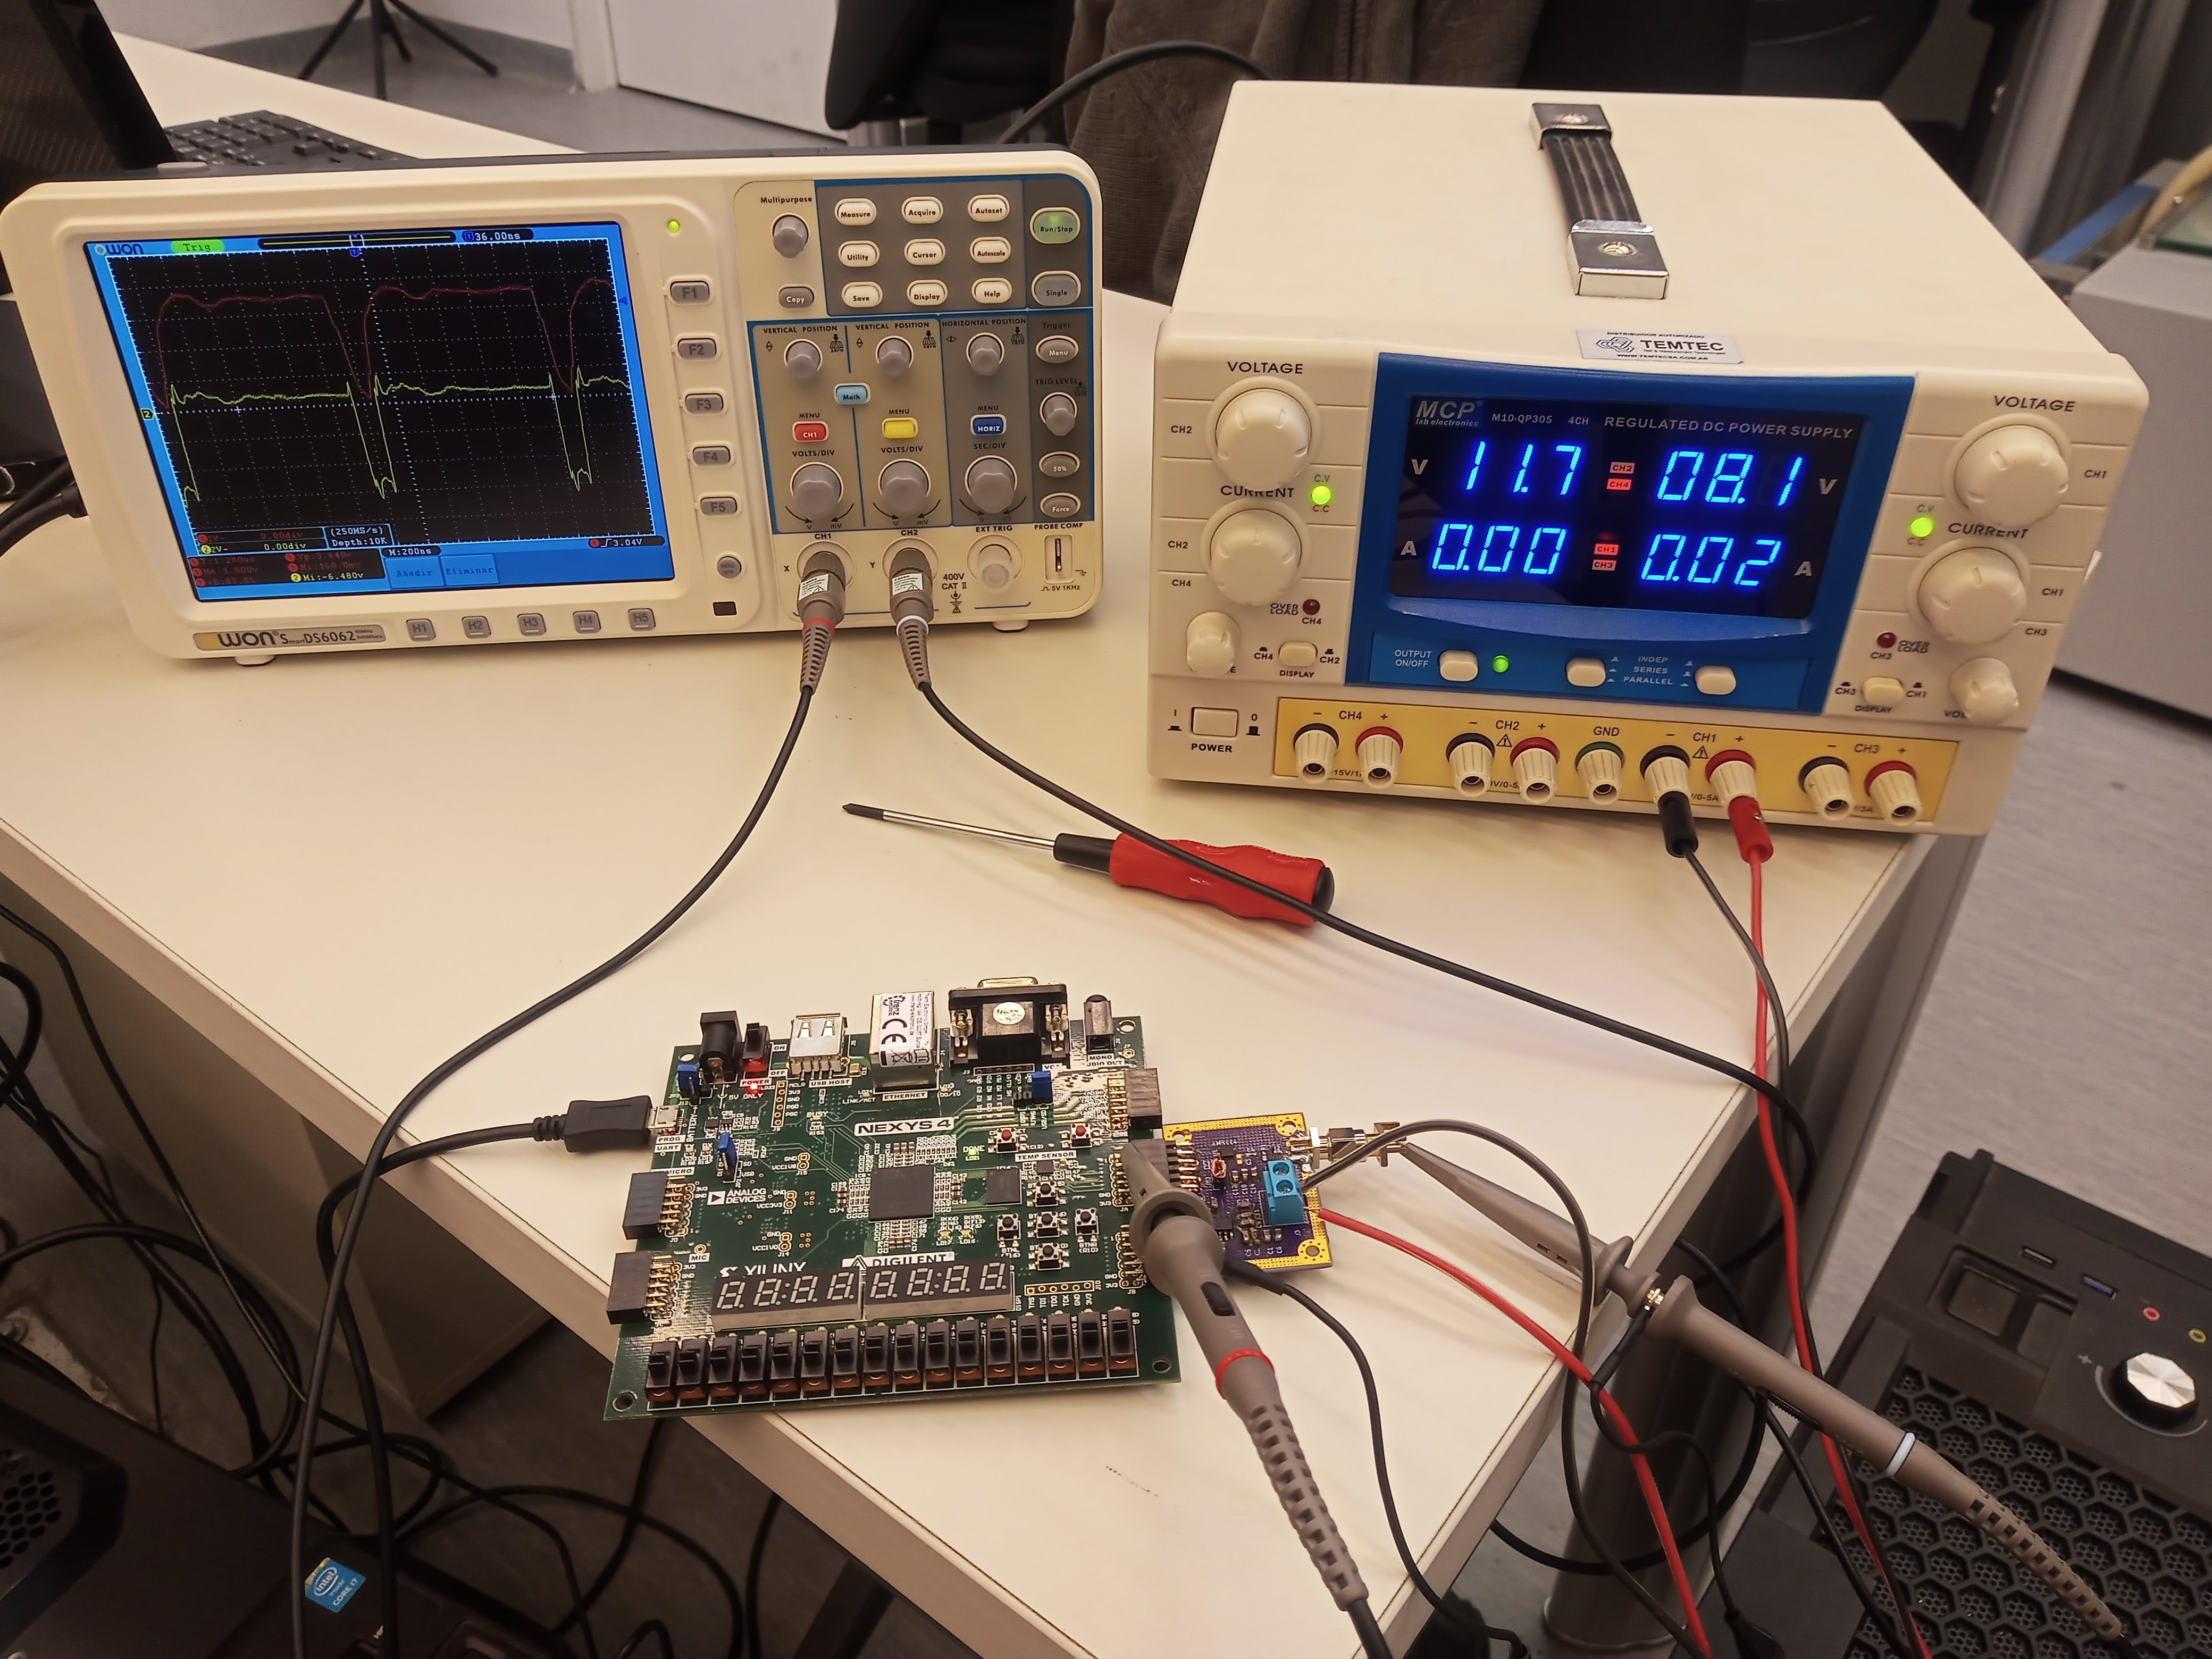
\includegraphics[width=0.4\textwidth]{images/banco_pre_mediciones.jpg}
    \caption{Banco de mediciones previas a la medición final del pulso.}
    \label{fig:banco_pre_mediciones}
\end{figure}

\subsection{Resultados}

En las figuras \ref{fig:mediciones_5v_50}, \ref{fig:mediciones_5v_70},
\ref{fig:mediciones_7v_50}, \ref{fig:mediciones_7v_60},
\ref{fig:mediciones_7v_70} pueden observarse los resultados en diversas capturas de pantalla
tomadas del osciloscopio.

Se observó en las mediciones una amplitud de pulso creciente con mayor ciclo de
trabajo y mayor amplitud de pulso, como era esperado. La menor amplitud de pulso
obtenida fue de \qty{380}{\milli\volt} para un $V_{cc}$ de \qty{5}{\volt} y un D
de \qty{50}{\percent}, y la mayor fue de \qty{1.12}{\volt} para un $V_{cc}$
de \qty{7}{\volt} y un D de \qty{70}{\percent}

En cuanto al ancho de pulso, se mantuvo aproximadamente constante en
\qty{160}{\pico\second}, al igual que los tiempos de crecimiento y
decrecimiento, que se mantuvieron constantes en \qty{90}{\pico\second}. Este
resultado es el esperado para un \textit{pulser} basado en un \textit{stub}, ya
que el ancho de pulso está determinado por el largo del \textit{stub}.

En la tabla \ref{tab:mediciones_resultados} pueden observarse los resultados
obtenidos. Para el ancho de banda, se utiliza el obtenido a partir de la
\textit{PSD} del pulso medido. En la sección \ref{sec:comp_simulacion} se
detalla cómo fue obtenido este valor.

\begin{figure}
  \centering
    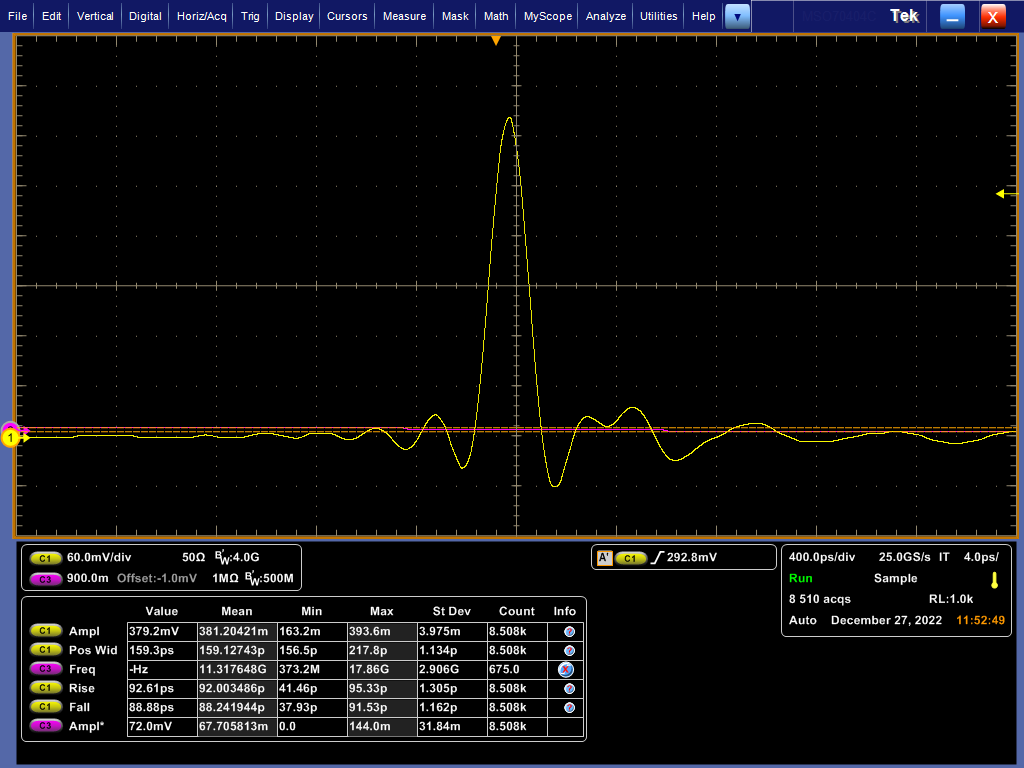
\includegraphics[width=0.6\textwidth]{images/mediciones/vcc_5v_duty_50.png}
    \caption{Salida @ $V_{cc}$ \qty{5}{\volt}, D \qty{50}{\percent} }
    \label{fig:mediciones_5v_50}
\end{figure}

\begin{figure}
  \centering
    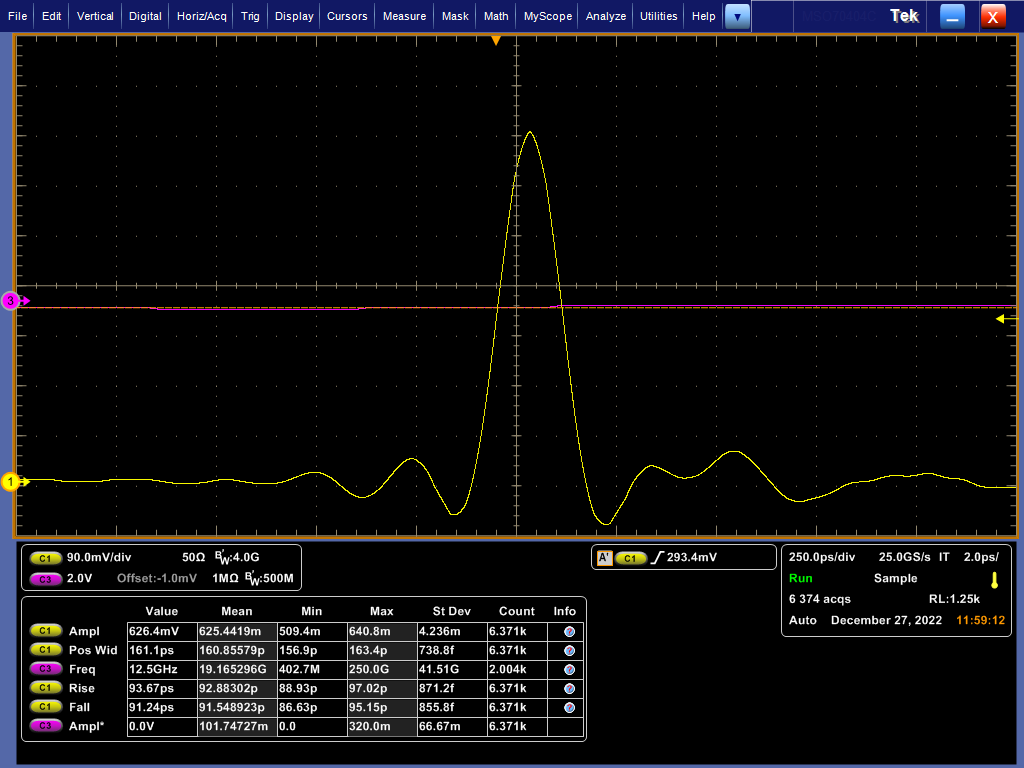
\includegraphics[width=0.6\textwidth]{images/mediciones/vcc_5v_duty_70.png}
    \caption{Salida @ $V_{cc}$ \qty{5}{\volt}, D \qty{70}{\percent} }
    \label{fig:mediciones_5v_70}
\end{figure}

\begin{figure}
  \centering
    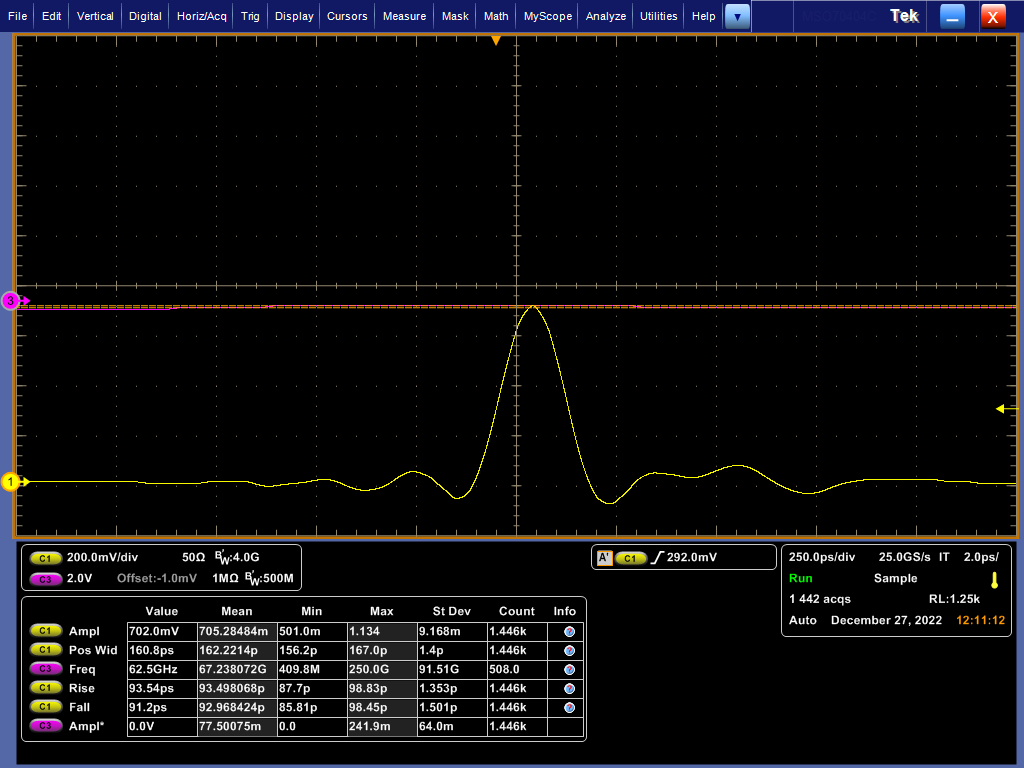
\includegraphics[width=0.6\textwidth]{images/mediciones/vcc_7v_duty_50.png}
    \caption{Salida @ $V_{cc}$ \qty{7}{\volt}, D \qty{50}{\percent} }
    \label{fig:mediciones_7v_50}
\end{figure}

\begin{figure}
  \centering
    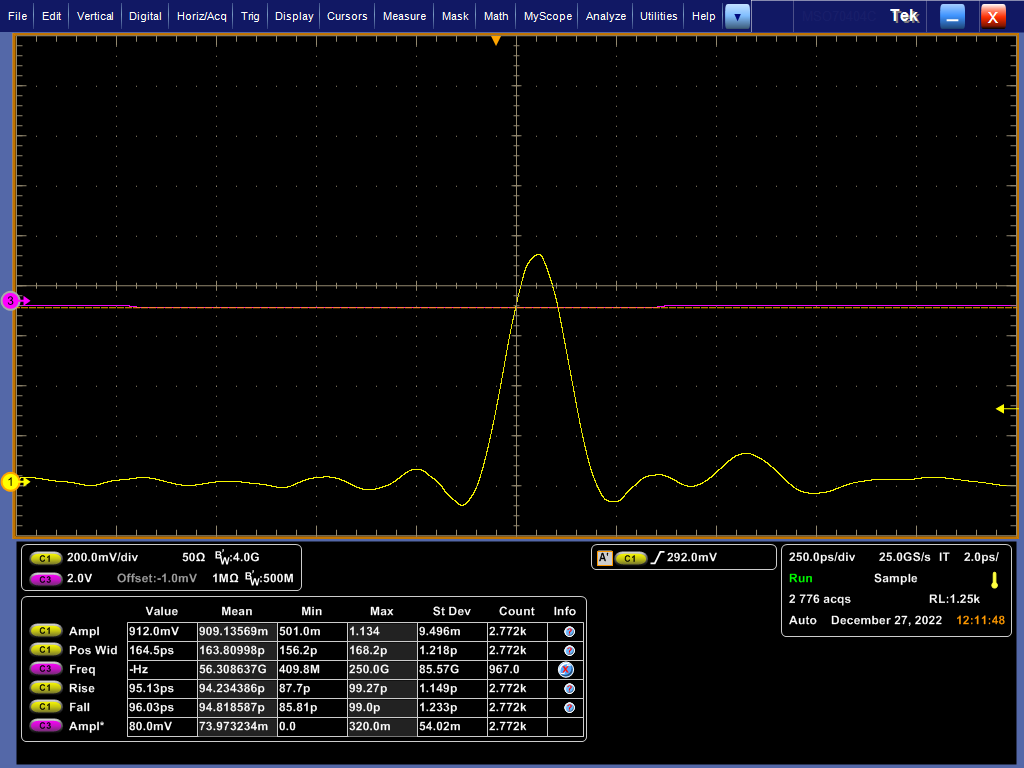
\includegraphics[width=0.6\textwidth]{images/mediciones/vcc_7v_duty_60.png}
    \caption{Salida @ $V_{cc}$ \qty{7}{\volt}, D \qty{60}{\percent} }
    \label{fig:mediciones_7v_60}
\end{figure}

\begin{figure}
  \centering
    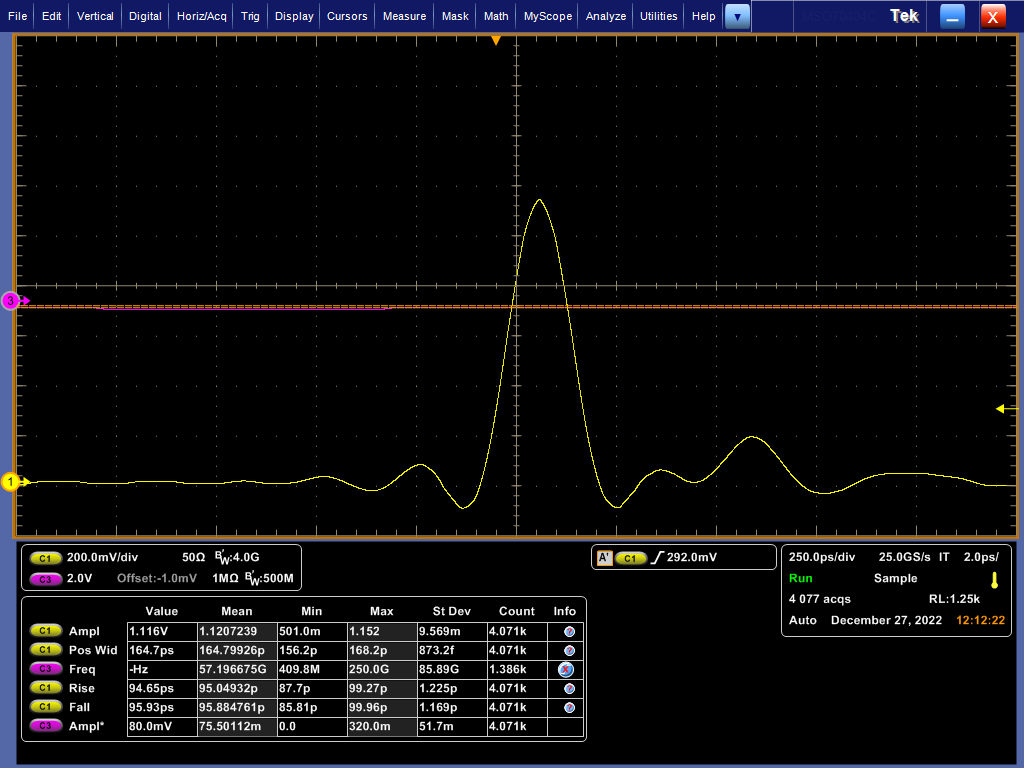
\includegraphics[width=0.6\textwidth]{images/mediciones/vcc_7v_duty_70.png}
    \caption{Salida @ $V_{cc}$ \qty{7}{\volt}, D \qty{70}{\percent} }
    \label{fig:mediciones_7v_70}
\end{figure}

\begin{table}
\centering
\begin{tabular}{ccccccc}
\hline
$V_{cc}$ [\unit{\volt}] & $D$ [\unit{\percent}] & $A$ [\unit{\volt}] &
    $FWHM$ [\unit{\pico\second}] & $\qty{3}{\dB} \ B$ [\unit{\giga\hertz}]& $t_r$
    [\unit{\pico\second}]& $t_f$ [\unit{\pico\second}]\\
\hline
5 & 50 & 0.380 & 159 & 7.5 & 93 & 88 \\
5 & 70 & 0.625 & 161 & 3.6 & 93 & 91 \\
7 & 50 & 0.702 & 162 & 4   & 93 & 93 \\
7 & 60 & 0.909 & 164 & 4   & 94 & 95 \\
7 & 70 & 1.120 & 165 & 2.8 & 95 & 96 \\
\hline
\end{tabular}
\caption{Resultados de mediciones.}
\label{tab:mediciones_resultados}
\end{table}

\subsubsection{Comparación con simulación}
\label{sec:comp_simulacion}

En las figuras \ref{fig:plots_5v_50} a \ref{fig:psd_7v_70} pueden observarse los resultados de las
mediciones obtenidas superpuestos con los resultados de simulación para las mismas condiciones de
trabajo (amplitud de alimentación y ciclo de trabajo).

Para las simulaciones, se toman dos resultados:

\begin{itemize}
    \item Una simulación ``ideal'', indicada como ``esquemático ideal'' en las
      leyendas, que se corresponde a una simulación sin contemplar parásitos de
      ningún tipo.
    \item Una simulación ``real'', en las leyendas ``Layout'', una simulación en
      la que se extrajeron previamente los efectos parásitos del \textit{PCB}
      mediante una simulación electromagnética y se incorporaron en la
      simulación del pulso.
\end{itemize}

Se realizan las comparaciones en el dominio del tiempo y de la frecuencia. Las
comparaciones en el dominio del tiempo consisten en la superposición del pulso
medido con los simulados. Para las comparaciones en el dominio de la frecuencia,
se calculó el espectro de cada una de las formas de onda del dominio del tiempo.
Para reducir el \textit{leakage} espectral, se utilizó una ventana de
\textit{Hanning} \cite{oppenheim1999dsp}.

En el dominio del tiempo, se observa una buena coincidencia entre la amplitud de
los pulsos y el ancho. Se observa una diferencia en el \textit{ringing} de
ambos.  Las simulaciones prácticamente no presentan oscilaciones alrededor del
pulso, mientras que las mediciones las presentan tanto previa como
posteriormente.  También se observa un segundo pulso de menor amplitud siguiendo
al primero.

Como causa de estas discrepancias, se descarta un efecto del \textit{PCB} no
modelado, ya que los parásitos de esta estructura fueron extraídos por una
simulación electromagnética, y sus efectos contemplados en las simulaciones del
\textit{layout}.

Estas  discrepancias sugieren una limitación en el modelado de alguno de los 
dispositivos, tanto el SRD como el Schottky. Las simulaciones predijeron correctamente
la amplitud y el ancho de los pulsos resultantes, pero fallaron en predecir 
el ringing y el pulso secundario.

\begin{figure}
  \centering
    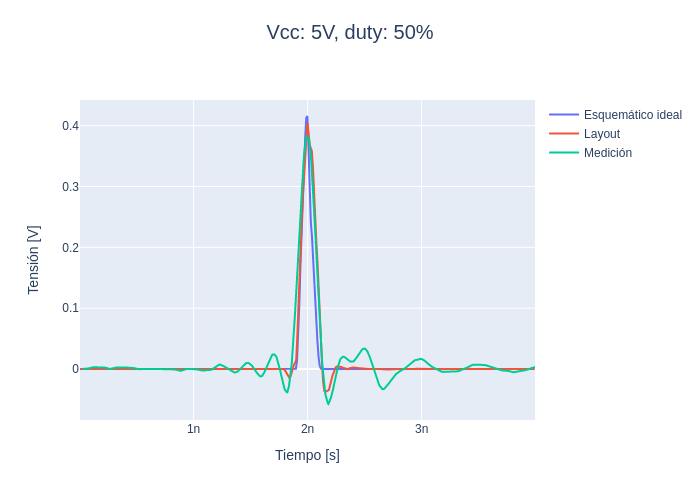
\includegraphics[width=0.6\textwidth]{images/plots/Vcc_5V_duty_50_time_domain.png}
    \caption{Pulso @ $V_{cc}$ \qty{5}{\volt}, D \qty{50}{\percent} }
    \label{fig:plots_5v_50}
\end{figure}

\begin{figure}
  \centering
    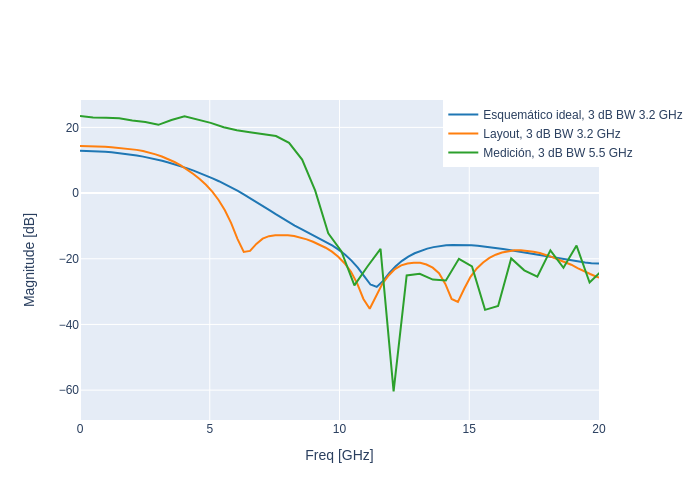
\includegraphics[width=0.6\textwidth]{images/plots/Vcc_5V_duty_50_psd.png}
    \caption{PSD @ $V_{cc}$ \qty{5}{\volt}, D \qty{50}{\percent} }
    \label{fig:psd_5v_50}
\end{figure}

\begin{figure}
  \centering
    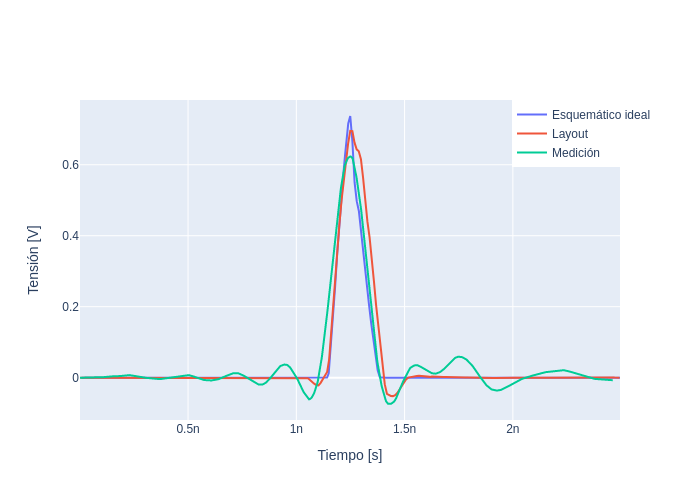
\includegraphics[width=0.6\textwidth]{images/plots/Vcc_5V_duty_70_time_domain.png}
    \caption{Pulso @ $V_{cc}$ \qty{5}{\volt}, D \qty{70}{\percent} }
    \label{fig:plots_5v_70}
\end{figure}

\begin{figure}
  \centering
    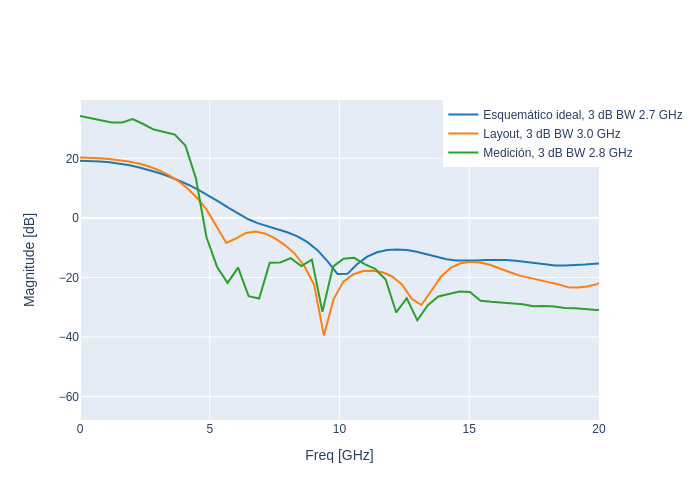
\includegraphics[width=0.6\textwidth]{images/plots/Vcc_5V_duty_70_psd.png}
    \caption{PSD @ $V_{cc}$ \qty{5}{\volt}, D \qty{70}{\percent} }
    \label{fig:psd_5v_70}
\end{figure}

\begin{figure}
  \centering
    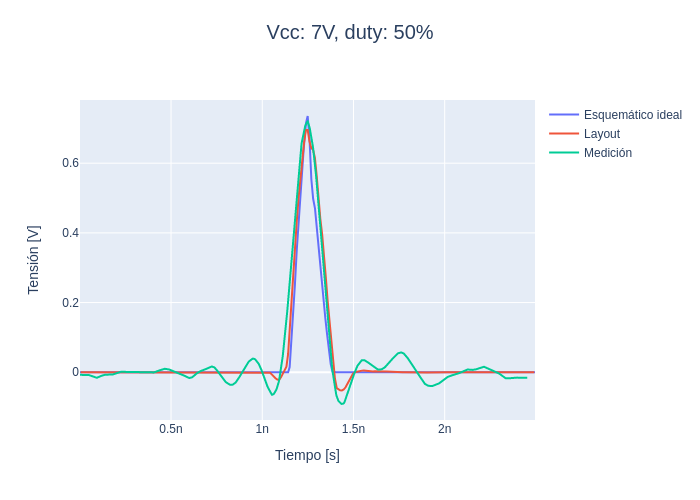
\includegraphics[width=0.6\textwidth]{images/plots/Vcc_7V_duty_50_time_domain.png}
    \caption{Pulso @ $V_{cc}$ \qty{7}{\volt}, D \qty{50}{\percent} }
    \label{fig:plots_7v_50}
\end{figure}

\begin{figure}
  \centering
    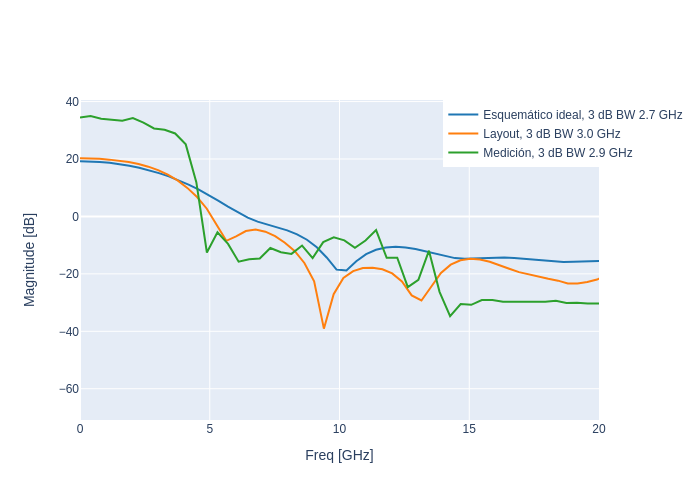
\includegraphics[width=0.6\textwidth]{images/plots/Vcc_7V_duty_50_psd.png}
    \caption{PSD @ $V_{cc}$ \qty{7}{\volt}, D \qty{50}{\percent} }
    \label{fig:psd_7v_50}
\end{figure}

\begin{figure}
  \centering
    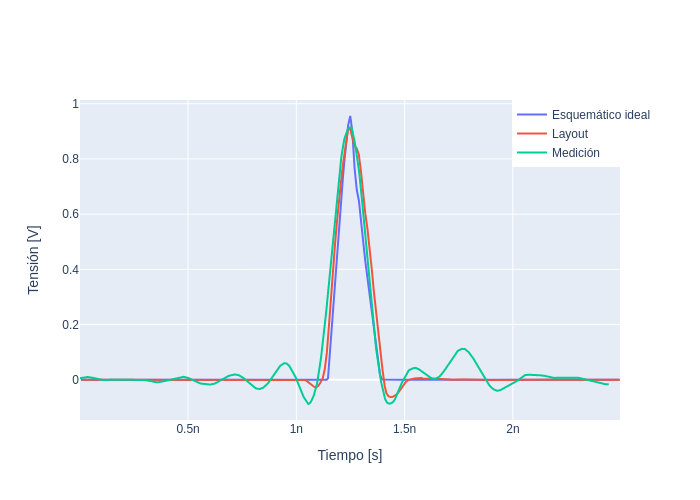
\includegraphics[width=0.6\textwidth]{images/plots/Vcc_7V_duty_60_time_domain.png}
    \caption{Pulso @ $V_{cc}$ \qty{7}{\volt}, D \qty{60}{\percent} }
    \label{fig:plots_7v_60}
\end{figure}

\begin{figure}
  \centering
    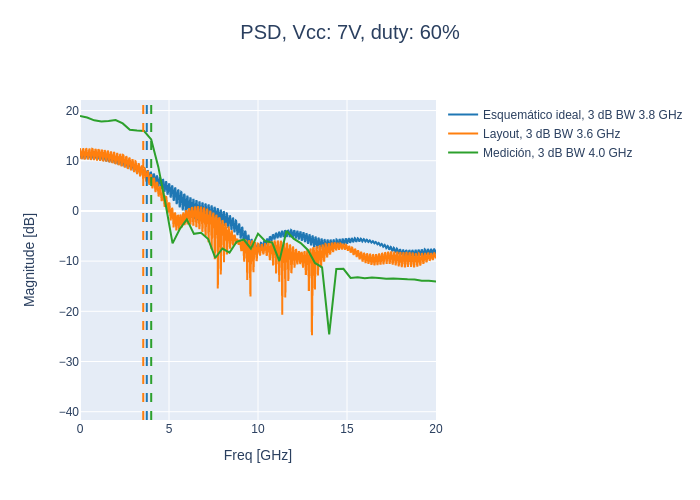
\includegraphics[width=0.6\textwidth]{images/plots/Vcc_7V_duty_60_psd.png}
    \caption{PSD @ $V_{cc}$ \qty{7}{\volt}, D \qty{60}{\percent} }
    \label{fig:psd_7v_60}
\end{figure}

\begin{figure}
  \centering
    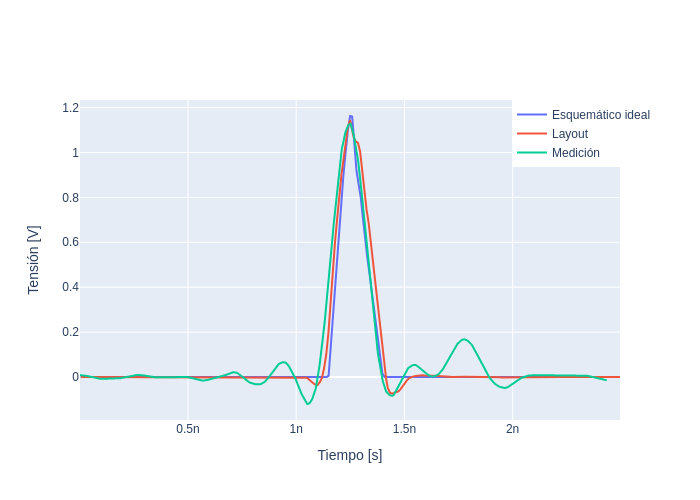
\includegraphics[width=0.6\textwidth]{images/plots/Vcc_7V_duty_70_time_domain.png}
    \caption{Pulso @ $V_{cc}$ \qty{7}{\volt}, D \qty{70}{\percent} }
    \label{fig:plots_7v_70}
\end{figure}

\begin{figure}
  \centering
    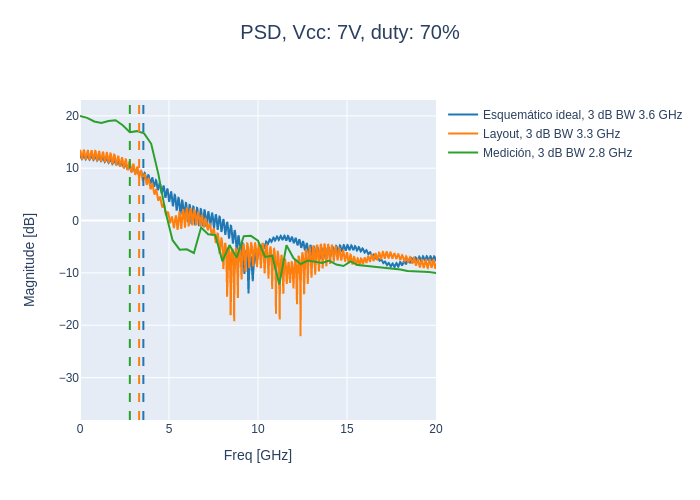
\includegraphics[width=0.6\textwidth]{images/plots/Vcc_7V_duty_70_psd.png}
    \caption{PSD @ $V_{cc}$ \qty{7}{\volt}, D \qty{70}{\percent} }
    \label{fig:psd_7v_70}
\end{figure}

\subsubsection{Comparación con resultados de la literatura}

En la tabla \ref{tab:resultados_literatura} se resumen resultados reportados para generadores de
pulsos \textit{UWB} en la literatura. En la figura \ref{fig:scatterplot_literature} se observan
los valores de amplitud y duración reportados en un gráfico de dispersión.

\begin{table}
  \begin{threeparttable}[b]
    \caption{Resultados reportados en la literatura}
    \label{tab:resultados_literatura}
    {\footnotesize
    \begin{tabular}{ccccccccc}
        \hline
        Referencia & $A$ [\unit{\volt}] & $FWHM$ [\unit{\pico\second}] &
        Bal \tnote{a} & Bias & Dispositivos & $V_{cc}$ [\unit{\volt}] & $V_{in}$ [\unit{\volt}] & $PRF$ [\unit{\mega\hertz}] \\
        \hline
        \cite{rulikowski2004} & \num{\pm 0.896}, \num{\pm 1.6} \tnote{b} & 335, 511 & Sí & Int & SRD & 5 & TTL & 50 \\
        \cite{protiva2009} & \num{-7.5} & 110 & No & Ext & SRD+3TBJ+SD & 12 & TTL & 5 \\
        \cite{kamal2014} & \num{0.8} & 170 & No & Int & SRD & 4 & 4 & 10 \\
        \cite{han2002} & \num{0.2} & 300 & No & Ext & SRD+2SD & ? & ? & 10 \\
        \cite{han2005} & \num{-6}, \num{-4} & 150 & No & Int & SRD+L & ? & 5 & 12 \\
        \cite{oloumi2018} & \num{1.27} \tnote{c} & 286 & No & Int & 2SRD+L & 10 & 10 \tnote{d} & ? \\
        \textbf{Este trabajo} & \num{1.12} & 165 & No & Int & SRD+SD & 7 & CMOS  &
        \num{10} \\
    \end{tabular}
}
   \begin{tablenotes}
     \item [a] \textit{Balanceado}.
     \item [b] la publicación presenta dos resultados, correspondientes a
       circuitos con componentes concentrados y distribuidos.
     \item [c] la publicación presenta múltiples resultados, se muestran
       los mejores.
     \item [d] la señal de entrada es senoidal.
   \end{tablenotes}
  \end{threeparttable}
\end{table}

\begin{figure}
\centering
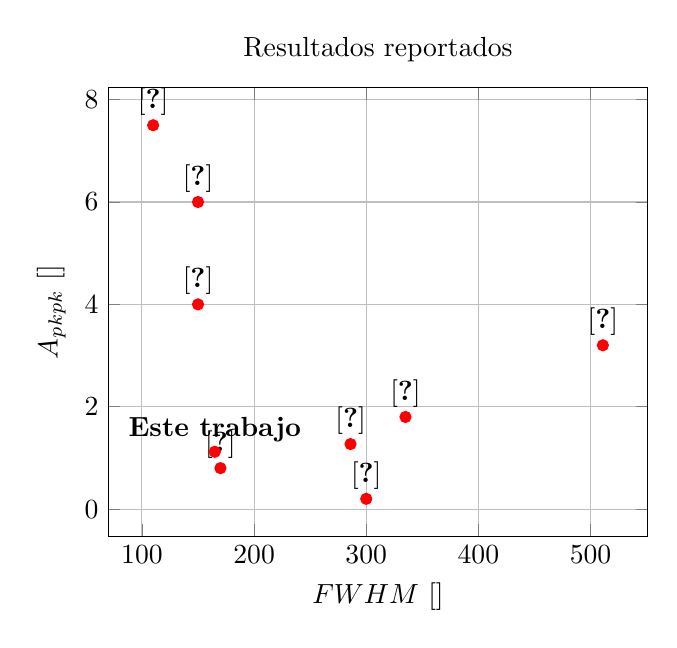
\begin{tikzpicture}
  \begin{axis}[
    xlabel={$FWHM$ [\unit{\pico\second}]},
    ylabel={$A_{pkpk}$ [\unit{\volt}]},
    title=Resultados reportados,
    grid=both
    ]
    \addplot[
        scatter/classes={a={blue}, b={red}},
        scatter, mark=*, only marks, 
        scatter src=explicit symbolic,
        nodes near coords*={\Label},
        visualization depends on={value \thisrow{label} \as \Label} %<- added value
    ] table [meta=class] {
        x   y       class   label
        511 3.2     b       {\cite{rulikowski2004}}
        335 1.8     b       {\cite{rulikowski2004}}
        110 7.5     b       {\cite{protiva2009}}
        170 0.8     b       {\cite{kamal2014}}
        300 0.2     b       {\cite{han2002}}
        150 6       b       {\cite{han2005}}
        150 4       b       {\cite{han2005}}
        286 1.27    b       {\cite{oloumi2018}}
        165 1.12    b       {\textbf{Este trabajo}}
    };

  \end{axis}
\end{tikzpicture}
  \caption{Diagrama de dispersión de resultados reportados.}
  \label{fig:scatterplot_literature}
\end{figure}

En cuanto a los resultados reportados en este trabajo, se obtuvo uno de los
anchos de pulso más bajos, existiendo otros trabajos que reportan el mismo o
menor ancho de pulso con mayor amplitud, pero también mayor complejidad. Otra
característica a destacar es la simplicidad del diseño implementado, tanto en
cantidad de componentes activos, como en requisitos de fuente de alimentación y
pulso de entrada.

En \cite{rulikowski2004} se presenta un diseño compuesto de un solo SRD en el
que se desarrolla un pulso balanceado a la salida. Se presentan dos diseños, uno
con componentes distribuidos y otro con componentes concentrados. En ambos casos
se obtienen amplitudes pico a pico de pulso mayores a las de este trabajo. Es
destacable que se obtienen mayores amplitudes usando una fuente de alimentación
menor, de \qty{5}{\volt}. En cuanto al ancho de pulso, ambos pulsos presentan
duraciones mayores que las de nuestro trabajo. En cuanto a la complejidad, el
\textit{pulser} está implementado solamente con 1 \textit{SRD} y componentes
distribuidos o concentrados, dependiendo de la versión, por lo que es más simple
que nuestro trabajo. El \textit{driver} presenta la misma complejidad en ambos
casos, ya que está implementado con un solo circuito integrado. Nuestro trabajo
presenta más versatilidad, ya que la amplitud de la fuente de alimentación puede
variarse entre \qty{0}{\volt} y \qty{30}{\volt}, mientras que el integrado
utilizado en el driver de \cite{rulikowski2004} trabaja con \qty{5}{\volt}
fijos.

En \cite{protiva2009} se reporta un resultado de gran amplitud y duración de
pulso menor a la de este trabajo. La complejidad del diseño implementado es
mucho mayor: necesita una alimentación de \qty{12}{\volt} y
una corriente de \textit{bias} externa, y la etapa \textit{driver} está
implementada con 3 TBJs, frente a 1 solo \textit{gate driver} en nuestro
trabajo.

En \cite{kamal2014} el pulso reportado es de características muy similares a las
de nuestro trabajo.  La duración del pulso es prácticamente la misma, mientras
que en amplitud nuestro trabajo logró una mayor en un \qty{40}{\percent}.
Nuestro trabajó logró para el \textit{pulser} una complejidad menor a la
reportada en \cite{kamal2014}, ya que en nuestro caso omitimos la red RC y el
atenuador. En cuanto a etapa \textit{driver}, \cite{kamal2014} no presenta
ninguna, en los resultados se reporta haber utilizado como entrada al
\textit{pulser} un pulso bipolar.

En \cite{han2002} el generador presentado desarrolla pulsos monociclo, que son
la primera derivada de un pulso gaussiano. Nuestro trabajó logro una amplitud de
pulso mayor y también una duración de pulso menor. No se especifica el valor de
amplitud de señal de entrada utilizado. La entrada al circuito es bipolar, y no
se incluye un \textit{driver} de adaptación de pulso. La complejidad del
generador descripto es mayor que la de este trabajo, utilizando bias externo, un
diodo SRD, dos Schottky y una red RC. Sin embargo, el generador de
\cite{han2002} implementa un monociclo que es una derivada de un pulso gaussiano
como el desarrollado en nuestro trabajo, por lo que es natural que la
complejidad sea mayor.

El resultado reportado en \cite{han2005} consiste en pulsos de mayor amplitud y
menor duración a los de nuestro trabajo. En ambos casos, el pulser se encuentra
acoplado por \textit{AC}, lo que vuelve más complejo el diseño.  Se presentan
dos generadores, uno con línea de transmisión, y otro con un inductor, que
utiliza al SRD en paralelo. El diseño con inductor es más complejo, ya que este
se encuentra en el camino del pulso por lo que debe ser seleccionado con
cuidado. En ambos casos se utiliza una red RC paralelo, mientras que en nuestro
trabajo no.

El resultado de \cite{oloumi2018} consiste en un pulso de mayor amplitud y mayor
ancho al de nuestro trabajo. La complejidad del diseño es mayor, ya que utiliza
dos SRD y un inductor que se encuentra en el camino de alta frecuencia, por lo
que es costoso de seleccionar. La señal de entrada es una senoidal, que para el
contexto en el que desarrollamos nuestro generador, es más costosa de conseguir,
ya que requiere algún DAC, frente a la excitación de nuestro generador que es
una señal cuadrada, fácilmente obtenible como salida digital de una FPGA o
microcontrolador.
